\documentclass{whutmod}
\usepackage{metalogo}
\usepackage{cases}
\usepackage{cite}
\usepackage{shorttoc}
\usepackage{longtable,booktabs}
\usepackage{float}
\usepackage{algorithm}  
\usepackage{algpseudocode}  
\usepackage{amsmath}  
\usepackage{textcomp}
\usepackage{caption}
\usepackage{subfigure}
\usepackage{threeparttable}
\renewcommand{\algorithmicrequire}{\textbf{Input:}}  % Use Input in the format of Algorithm  
\renewcommand{\algorithmicensure}{\textbf{Output:}} % Use Output in the format of Algorithm  
\bibliographystyle{ref}
\team{20}	% 组号
\membera{张方祚}
\joba{编程}
\memberb{彭译萱}
\jobb{建模}
\memberc{刘佳迎}
\jobc{建模}

\title{基于NSGA和Pareto法则的动态多目标装载模型}
\tihao{7} % 题号

\begin{document}

\maketitle

\begin{abstract}
    \keywords{  
    疾病预测\quad
    灰色预测\quad

	}
\end{abstract}

\tableofcontents
\thispagestyle{empty}
\newpage
\setcounter{page}{1}

\section{问题重述}
\subsection{问题背景}

传染病是由各种病原微生物或寄生虫感染后,能够在人与人、人与动物及动物之间互相传播的一类疾病。在已经得知的传染病中,一部分传染性疾病会对人造成严重的伤害,流行性非常高,很多国家借助政府的力量进行监控,严防造成严重的后果,避免疫情的扩大。
卫生防疫部门要准确掌握,以便于及时采取应对措施。

我国法定传染病监测建立,任务是被动地收集、汇总全国人口法定传染病数据,对传染病流行期进行监测,作出迅速反应。
该系统是重要的宏观法定传染病监测系统,在预防与控制传染病、应对传染病和突发公共卫生事件以及防控传染病因素带来的社会安全事件的方面取得了积极良好的成效。

在传染病预测中,如何根据历史数据预测未来患病人数,并提高预测精确度,具有重要意义。请根据某种传染病按照年份、四种诊断方法、地区和职业的划分得到的发病人数和死亡人数汇总数据,解决以下问题:

\subsection{问题的提出}
\textbf{问题1:}分析该传染病在整个国家从2004-2016年的流行病学变化趋势,并对2019年全国感染该疾病的发病人数和死亡人数作出预测;

\textbf{问题2:}收集2004年-2016年以三年为时间间隔的传染病发病率和死亡率,给出的不同地区和职业分类统计的传染病数据,建立传染病传播的数学模型,并预测2019年传染病防控排名前3位的重点区域和重点人群。

\textbf{问题3:}经济发展与疾病传播程度在一定程度上具有相关性,添加经济发展影响的指标,对该传染病预测模型进行改进,并分析你的结论。

\textbf{问题4:}结合流行病历史数据和2019年预测数据,给卫生健康委员会相关部门写一封公开信,提出能够有效防控疾病疫情的建议和看法。
\newpage 

\section{模型的假设}
\begin{itemize}
    \item 比例系数不变。即传染系数、病毒潜伏期和恢复系数为常数。
    \item 传染病的传播一个测量周期(一年)内完成,不会对发病人数和死亡人数的统计产生影响。
    \item 总人数不变。即考虑在一个封闭的区域,忽略人口的迁移因素。
\end{itemize}

\section{符号说明}
\begin{table}[!htbp]
    \centering
    \begin{threeparttable}[b]
    \caption{符号说明}
    \label{tab001} 
	\begin{tabular}{ccccc}
		\toprule[1.5pt]
        \multicolumn{1}{m{3cm}}{\centering 符号} & \multicolumn{1}{m{6cm}}{\centering 定义} \\%第一列占3cm,第二列占6cm并且都居中
        \midrule[1pt]
        $b_i$ & 第$i$年的发病率 \\
        $B_i$ & 第$i$年的发病人数 \\
        $sum_i$ & 第$i$年的总人数 \\
        $d_i$ & 第$i$年的死亡率 \\
        $D_i$ & 第$i$年的死亡人数 \\ 
        $M_{ij}$ & 第$i$种诊断方案第$j$年的发病人数 \\
        $N_{ij}$ & 第$i$种诊断方案第$j$年的死亡人数 \\
        $m_{ij}$ & 第$i$种诊断方案第$j$年的发病人数占比 \\
        $n_{ij}$ & 第$i$种诊断方案第$j$年的死亡人数占比 \\
		\bottomrule[1.5pt]
    \end{tabular}
    \begin{tablenotes}
        \item 注:其他未出现符号在文中对应部分详细注明。
      \end{tablenotes}
     \end{threeparttable}
\end{table}
\newpage

\section{问题分析}
\subsection{问题一分析}
问题一要求根据前13年传染病的历史数据,对2019年传染病的发病人数和死亡人数作出预测。
鉴于题目所给数据是全国四种诊断方案的发病人数和死亡人数,为了提高数据模拟的精度,我们对四种诊断方案分别拟合,通过人数占比求出全国的发病人数和死亡人数。

\subsection{问题二分析}
问题二在问题一的基础上,对全国传染病的患病人数和死亡人数作出关于省份和不同类型人群的划分,增加了数据的精确度,同时也对预测模型的准确度要求更高。
考虑到传统的传染病模型以一天或者一周作为单位时间,不适用于以三年为单位时间的预测模型,我们采用有效筛选人群和区域划分的方式进行预测。

\subsection{问题三分析}
与问题二相比较,问题三需要考虑城市经济发展对传染病的影响,因此需要选取同时代表经济增长和医疗条件的的城市指标。
最后我们选取了每个省份的居民消费支出、医疗卫生机构这些具有代表性的数据数作为评价传染病模型的指标。

\subsection{问题四分析}
结合传染病历史数据和2019年的预测数据,分析病情的地区时空传播特点,以及在各个类型人群中的发病情况,对市政府给出了合理有效的建议。

\section{基于改进的P-GM(1,1)灰色预测传染病预测模型}
\subsection{问题分析}
问题一需要根据题目所给的在四种诊断方案下全国发病人数和死亡人数的历史数据,对2019年作出预测。由于传染病在传播过程中病菌会不断发生演变,城市经济发展使得医疗条件不断提高,这些都会对传染病的传播造成影影响。
因此可以认为,距离预测时间点越近的历史数据对预测值影响越大。在此理论基础上,我们建立了基于改进灰色预测模型的传染病预测模型,对2017-2019年的发病人数和死亡人数作出预测。

\subsection{预备工作}
\subsubsection{数据预处理}
我国2004-2006年人口总数不断增加,人口密度越来越大,传染病的发病人数和死亡人数的变化可能会受到人口基数影响。为了消除该影响,求解过程中将发病人数和死亡人数转化为发病率和死亡率,其转化公式如下:
\begin{equation}
    b_i=\frac{B_i}{sum_i},
\end{equation}
\begin{equation}
    d_i=\frac{D_i}{B_i},
\end{equation}
其中,$b_i$为第$i$年的发病率,$B_i$为第$i$年的发病人数,$sum_i$为第$i$年全国总人数。$d_i$为第$i$年的死亡率,$D_i$为第$i$年的死亡人数。

\subsubsection{变化趋势分析}
以全国为最小单位观察,我国2004-2016年流行病平均发病率为7.56\textperthousand,平均死亡率为2.77\textperthousand。
\begin{figure}[H]
    \centering
    \subfigure[四种诊断方法的发病率]{
    \begin{minipage}[t]{0.5\linewidth}
    \centering
    
\includegraphics[width=.9\textwidth]{1.png}
    \end{minipage}%
    }%
    \subfigure[四种诊断方法的死亡率]{
    \begin{minipage}[t]{0.5\linewidth}
    \centering
    
\includegraphics[width=.9\textwidth]{2.png}
    \end{minipage}%
    }%
    \centering
    \caption{发病率和死亡率比较}
\end{figure}
通过分析图 1 中13年间传染病发病率趋势可发现发病率呈现先升后降,总体下降,略有波动的趋势。2005年达到最高点,2016年达到最低点。其中2004-2005年的平均发病率为8.55\textperthousand,2006-2016年的平均发病率为7.39\textperthousand。

通过分析13年间传染病的死亡率趋势可发现其与发病率趋势大致相同,同样呈现先升后降的趋势。2004年为最低点,2009年达到最高点。其中2004-2009年的平均死亡率为2.70\textperthousand,2010-2016年的平均死亡率为2.82\textperthousand。

对A、B、C、D四种诊断方法分析比较后发现,方法A的死亡率呈现先上升后下降的趋势,说明该方法随着时间不断发展,疗效不断提高。作为市场占比相加超过60\%的诊断法方法B和D,其发病占比和死亡占比变化波动不大,成为我国对此种流行病诊断治疗的主要方法。
作为应用范围第二广的诊断方法C,死亡率呈现总体上升的趋势,说明此种方法效果不理想,当科技发展到一定水平可以考虑放弃此种诊断方案。

\subsubsection{灰色系统理论}
灰色系统以部分信息已知、 部分信息未知的不确定性系统为研究对象,通过对已知信息的生成、开发,提取有价值的信息来进行预测,因而被广泛应用于通过历史数据预测未来数据的情景。其建模不依赖于数据的原始信息。

其建模机理如下:设原始序列$X^{(0)}=\{x^{(0)}(1),x^{(0)}(2),\dots,x^{(0)}(N)\}$,其中$x^{(0)}(i)\geq 0$,$i=1,2,\dots,N$。对原始序列进行累加得到$x^{(1)}(j)=\sum_{i=1}^jx^{(0)}(i)$,GM(1,1)的差分形式为:
\begin{equation*}
    x^{(0)}(j)=az^{(1)}(j)=b,
\end{equation*}
其中,$a$是发展系数,$b$是灰色作用量,$z^{(1)}(j)=\frac12[x^{(1)}(j-1)+x^{(1)}(j)]$。
得到灰色预测公式为:
\begin{equation*}
    x^{(0)}(j+1)=x^{(1)}(j+1)-x^{(1)}(j)=1-e^a)[x^{(1)}(1)-\frac{b}{a}]e^{-aj},j=0,1,\dots,N-1.
\end{equation*}

\subsection{基于改进的P-GM(1,1)传染病预测模型的建立}
通过对历史数据进行累加,我们发现序列呈现出整体的灰指数规律,在此基础上分别构建灰色微分方程,并对每种诊断方法的发病率求解计算每种诊断方法每年的发病人数和患病人数
,发病人数占比和患病人数占比。
因此,对四种诊断方案分别预测传染病的发病人数和死亡人数,并通过四种方案对全国传染病影响的占比对模型进行修正。
\begin{equation}
    m_{ij}=\frac{M_{ij}}{\sum_{i=1}^4M_{ij}},
\end{equation}
\begin{equation}
    n_{ij}=\frac{N_{ij}}{\sum_{i=1}^4N_{ij}},
\end{equation}
其中,$m_{ij}$表示第$i$种诊断方案第$j$年的发病人数占比,$n_{ij}$表示第$i$种诊断方案第$j$年的死亡人数占比。

为了减小预测误差,我们将四种诊断类型占比的变化趋势带入模型,并在GM(1,1)模型的基础上添加三次多项式回归模型对数据进行拟合优化\textsuperscript{\cite{bib:two}},
最终基于改进的P-GM(1,1)传染病预测模型的表达式为:
\begin{equation}
    x_{(0)}(i)=b_3[\bar x_{(0)}]^3+b_2[\bar x_{(0)}]^2+b_1[\bar x_{(0)}]+b_0
\end{equation}

其中$b_i(i=0,1,2,3)$为多项式系数,可由最小二乘法求解。$x_{(0)}(i)$序列为
预测发病人数序列、死亡人数序列、各诊断方法人数占比序列$X^{(0)}=\{x^{(0)}(1),x^{(0)}(2),\dots,x^{(0)}(N)\}$。

根据上述预测模型,带入$x_{(0)}(i)$序列计算出四种诊断方案的发病、死亡的占比和人数,进而求出四类全国总发病人数、死亡人数的预测值,并通过求平均的方法提高其综合预测精度,最终全国传染病发病人数$sum_m$的计算公式可表示为:
\begin{equation}
    sum_m=\frac{\sum_{i=1}^4M_{i2019}\textbackslash m_{i2019}}4,
\end{equation}
全国传染病总死亡人数$sum_n$的计算公式为:
\begin{equation}
    sum_n=\frac{\sum_{i=1}^4N_{i2019}\textbackslash n_{i2019}}4.
\end{equation}

\subsection{模型求解与结果检验}
\subsubsection{全国发病人数和死亡人数}

    step1:将预测发病人数序列、死亡人数序列、各诊断方法人数占比序列$X^{(0)}$带入$x_{(0)}$,使用最小二乘法求解各自的最优拟合系数

    step2:将拟合系数分别带入模型求解2017-2019年的A、B、C、D四种诊断方案的发病人数和死亡人数。

    step3:对A、B、C、D四种诊断方法分别得到全国传染病发病人数和患病人数的预测值求平均,进而减小预测误差。


经过改进的灰色预测模型得到2017-2019年该传染病的发病人数和死亡人数如下表所示:
\begin{table}[H]
    \caption{2017-2019年该传染病发病人数和死亡人数预测} \centering
    \begin{tabular*}{8cm}{cccccc}
        \toprule[1.5pt]
         & 2017年 & 2018年 & 2019年 \\
         \midrule[1pt]
         发病人数 & 821785 & 794996 & 776099 \\
         死亡人数 & & & \\
         \bottomrule[1.5pt]
    \end{tabular*}
\end{table}

\subsubsection{皮尔逊检验}
在预测全国传染病趋势模型中,发病率和死亡率都是按自然顺序进行的连续统计得到的,所以需要通过分析多个百分率是否与等级分层变量间存在关于时间的变化趋势。
现代医学对流行病常用的检验方式为皮尔逊(pearson)检验和CAT(Cochran-Armitage trend)检验\textsuperscript{\cite{bib:three}}。

皮尔逊方检验广泛应用于流行病学、遗传学和疾病发病率或死亡率等的时间趋势研究,能够比较理论频数和实际频数的吻合程度或拟合优度。其检验公式如下:
\centerline{\large{$\rho_{X,Y}=\frac{cov(X,Y)}{\sigma_x,\sigma_y}=\frac{E((X-\mu_X)(Y-\mu_Y))}{\sigma_x,\sigma_y}$}}
其中系数的取值总是在[-1,0]或者[0,1]之间,接近0 的变量无相关性,接近1或者-1被成为具有相关性。

我们对全国总体的发病率和死亡率,以及A、B、C、D四种诊断方法进行线皮尔逊检验,得到结果如下:
\begin{table}[H]
    \caption{全国指标和四种诊断方法关于发病率的皮尔逊检验} \centering
    \begin{tabular*}{13cm}{ccccccc}
    \toprule[1.5pt]
     & 全国 & 诊断方案A & 诊断方案B & 诊断方案C & 诊断方案D \\
     \midrule[1pt]
     r & -0.9729 & 0.8919 & -0.8682 & -0.7349 & 0.9876 \\
     p & 1.1045 & 9.6735 & 0.0002 & 0.0064 & 2.2166 \\
     \bottomrule[1.5pt]
    \end{tabular*}
\end{table}
由上表可得,对于发病率而言,全国数据和四种诊断方法关于皮尔逊检验得到的r值都接近于1或者-1,相关性显著。其中,全国数据、诊断方案B和诊断方法C的r值都为负数,因此这三组的数据和时间具有负相关性,说明该传染病得到了控制,且诊断方案C应用范围逐年缩小,与变化趋势中分析相同。
诊断方案A和诊断方案D的r值都接近于1,因此说明这两种方案随时间增长应用范围越来越广,也侧面证明了在变化趋势分析中D的市场占有率较高的原因。

\section{问题二模型的建立与求解}
\subsection{问题分析}
问题二根据职业和地区的不同,收集到传染病关于每个职业和每个地区的发病人数、死亡人数。与问题一不同的是,问题二的时间跨度为三年。鉴于典型的传染病模型时间跨度为天或月,因此,我们采用时间跨度更大的传染病预测模型对结果进行评估。

\subsection{预备工作}
\subsubsection{有效人群的筛选}
分析传染病发病人群的年龄分布特征发现,传染病的发病人数和死亡率受到不同人群类型影响较大。例如,散居儿童和离职退休人群属于免疫力较差的群体,传染病死亡率相比于其它年龄段也相对较高。
因此,我们对传染病的发病人数占比重新定义,其计算公式如下:
\begin{equation}
    a_{ij}=\frac{A_{ij}}{sum_j}
\end{equation}
其中,$a_{ij}$表示第$i$种人群第$j$年的发病率,$A_{ij}$表示第$i$种人群第$j$年的发病人数,$sum_{ij}$表示第$j$年所有发病人数。

对于传染病发病人数占比和死亡率较小的职业类别,在统计中可以视作为的小概率事件。
对此类职业人群进行数据预测时预测值较小,不影响最终传染病的防控排名结果。因此,我们通过设定阈值\textsuperscript{\cite{bib:four}}来向下筛选有效预测人群,只对对满足阈值要求的人群进行预测。

因此,对传染病发病人数占比选取2\%的阈值的人群进行预测,在统计年限中,当该类型的人群发病人数占比达到2\%时,选取此类人群作为预测对象。经计算得到选取了7个有效职业。

对传染病死亡选取1\textperthousand 的阈值人群进行预测,在统计年限中,当该类型的人群死亡率达到1\textperthousand 时,
选取此类人群作为预测对象。经计算得到10个有效职业。

分别关于发病人数占比和死亡率选取的有效职业如下表所示:
\begin{table}[H]
    \caption{有效人群类型的划分} \centering 
    \begin{tabular*}{14cm}{cccccccccc}
    \toprule[1.5pt]
    评价指标 & 有效人群类型 \\
    \midrule[1pt]
    \multirow{2}{*}{死亡率} & 幼托儿童、散居儿童、教师、医务人员、农民、牧民、渔民 \\
     & 公务人员及职员、家政家务及待业、海员及长途驾驶员 \\
     \hline
     \multirow{2}{*}{发病人数占比} & 学生、工人、民工、农民、公务人员及职员\\ 
      & 离退休人员、家政家务及待业 \\
    \bottomrule[1.5pt]
  \end{tabular*}
\end{table}
最后得到14种不同不同类型的人群进行传染病患病人数占比和死亡率的预测。

\subsubsection{地区的划分}
分析传染病模型的地区特征,发现传染病发病人数和死亡率除了受到人群类型影响较大外,还受到地区划分的影响\textsuperscript{\cite{bib:five}}。例如,上海市作为我国经济告诉发展的代表,人口密度大,有利于传染病的传播,死亡率和其它省份和地区相比也相对较高,周边省份或地区受到影响。

传染病的传播,分为省份自身和周边省份的影响。城市内部的人群密度、经济条件和年龄结构决定了传染病的传播速度和传播范围,在一些人口密度大的城市会对传染病的传播起促进作用。
同时,统一区域的周边城市也会对本城市传染病的传播造成影响,例如,当一个区域内有着消费水平和公共福利较好的城市,会带动周边城市的法阵,同时,当周边城市的人口患病时也会考虑到就近的水平较高的医院看病,此时减少了传染病的传播。

中国地理区域划分根据地理、气候、经济和行政管理等方面的特征,对全部国土区域按照其特点划分成七个大块,这种划分方式考虑了各个时代、研究重点、综合性与可比性,最后得到的划分的在一片区域内部的城市具有相似性。具体划分标准如下表4所示:

\begin{table}[H]
    \caption{根据地域特点的省份划分} \centering
    \begin{tabular*}{13cm}{ccccccc}
    \toprule[1.5pt]
     地区 & 省份 \\
     \midrule[1pt]
      华北 & 北京市、天津市、河北省、山西省、内蒙古 \\
      东北 & 辽宁省、吉林省、黑龙江 \\
      华东 & 上海市、江苏省、浙江省、安徽省、福建省、江西省、山东省 \\
      华中 & 河南省、湖南省、湖北省 \\
      华南 & 广西省、广东省、海南省 \\
      西南 & 重庆、四川省、贵州省、云南省、西藏 \\
      西北 & 陕西省、甘肃、宁夏、青海、新疆 \\
     \bottomrule[1.5pt]
    \end{tabular*}
\end{table}
根据相似点划分相同省份得到的区域如下图:
\begin{figure}[h]
    \centering
    
\includegraphics[width=.7\textwidth]{3.png}
    \caption{中国七大区域的划分}
\end{figure}

\subsection{问题二模型的建立}
\subsubsection{重点人群的预测模型}
问题二在问题一的基础上,添加了不同类型人群的划分。在找到可以进行有效预测的14种类型的职业后,与问题一的P-GM(1,1)模型相同,对每一种职业的的发病人数占比和死亡率进行预测。

传染病防控过程的衡量是综合指标的衡量,就需要分别对单因素进行评估后再进行复合指标衡量\textsuperscript{\cite{bib:eight}}。权重可以按照层次分析法确定,也可以依据决策人员的关注度而定。
由于问题二中的传染病的防控水平由两个指标决定:发病人数占比和死亡率,因此,重点人群复合决策模型可以简单表示为:
\begin{equation}
    fitness(COA x)=w_{1i}a_{ij}+w_{2i}d_{ij},
\end{equation}
其中,$w_{1i}$表示衡量第$i$种类型的人群对应相应发病人数占比$a_{ij}$的权重值,$w_{2i}$表示衡量第$i$种类型的人群对应相应死亡率$d_{ij}$的权重值,且有$w_{1i}+w_{2i}=1$。

考虑到采用两个指标对传染病重点人群进行排名,因此我们准备了三种权重方案描述两个指标对于总排名的重要程度。通过比较分别对两个指标的权重进行赋值如下:
$w_{1i}=0.7,w_{2i}=1-w_{1i}=0.3$时,表示进行排名决策时更偏向于发病人数占比较高的职业人群。
$w_{i1}=0.3,w_{2i}=1-w_{1i}=0.7$时,表明进行排名决策时更偏向于发病后死亡率较高的职业人群。
$w_{1i}=w_{2i}=0.5$时,即进行排名决策时发病人数占比和死亡率同样重要。

\subsubsection{重点区域的预测模型}
根据本问题传染病模型的时间跨度大,影响范围广,影响因素多的特点,我们提出了一种\textbf{小生境传染病传播模型}。

在生物学中,小生境是指在特定环境下的一种组织结构\textsuperscript{\cite{bib:nine}},具有相似特征和相似形状的物种聚集在一起,并在同类中交配繁衍后代,同时采用预选择、排挤、分享等机制个体间的交流和个体的演化。
该模型定义由小生境空间、个体邻域、个体状态和个体交流、演化规则构成。
当对中国各省份城市进行七大区域划分之后,可以把每个区域的省份构成一个小生境。即各个相近或相似的省、市级地区看做小生境的独立个体。
在每一个小生境内,保证个体优先在小生境中不断进化\textsuperscript{\cite{bib:ten}},即传染病只在小生境内传播,不考虑小生境外的个体对小生境内的个体影响。为了使模型更具有普适性和鲁棒性,一个个体可用数学符号表示为:
\begin{equation}
    A=(L,D,S,N,f),
\end{equation}
其中,$L=\{A_{ij},i,j\in Z\}\subset R$为小生境空间,表示所有个体$A$的集合,小生境空间中每个个体的属性是由$A_{ij...}$标记,个体属性个数由具体问题而定。首先我们将地区发病率与死亡率看做为小生境个体的两个基本属性。$D$为小生境空间的维数,由具体的结构确定。当个体属性状态为离散状态时,
可将$S=\{\varepsilon_1,\varepsilon_2,\dots,\varepsilon_p,p\in Z\}$是一个包含每个个体属性可能状态的离散集合,在$t$时刻每个个体的状态为$\varepsilon_t(A)$;当个体属性为连续状态时,我们将$S$定义为随着小生境迭代时个体属性值的变化量集合。
在传染病传播模型中可看做每年发病率、死亡率的变化量。
$N(A)$为个体$A$的邻域,是同一个小生境内的其他个体的集合,也是是影响该个体$A$属性值随小生境迭代(传染病传播)过程中变化的一组个体集合。
在传染病传播模型中可看做地区A所在的小生境内的其他地区集合。
$f$为个体间交流、个体自身演化规则。

个体交流规则是以个体当前属性和其领域个体属性为依据,确定下一时刻该个体属性值的变化规则,用以模拟其他合体对本体的影响。
个体自身演化规则是以个体当前属性为依据,确定下一时刻该个体属性值的变化规则,用以模拟本体自身属性对本体的影响。
变化规则可为:
\begin{equation}
f:S_i^{t+1}=f(S_i^N,S_t^N),
\end{equation}
其中,$S_i^{t+1}$为小生境每次迭代中个体$i$属性值的总变化量,对应城市的发病率、死亡率等属性值的变化量,
$S_i^N$为小生境每次迭代中个体$i$在演化规则下的属性值的总变化量,对应城市的发病率、死亡率等属性值的受其他个体条件因素影响的变化量。
$S_t^N$为小生境每次迭代中个体$i$在交流规则下的属性值的总变化量,对应城市的发病率、死亡率等属性值的受自身条件因素影响的变化量。

本问题求解时,将传染病的传播过程定义为小生境内的个体交流、演化的过程,发病率和死亡率随每年发生的变化看做小生境迭代过程中个体属性的变化。
因此只需要确定小生境内个体属性的变化规则即可对传染病的传播进行仿真,首先我们以小生境的基本属性发病率、死亡率为基础,通过傅里叶变化确定了小生境个体的基本变化规则:

\begin{equation*}
    f_q=k_1cos(\omega_a\alpha_b)+k_2sin(\omega_a\alpha_b)+2k_3cos(2\omega_a\alpha_a)+2k_4cos(2\omega_b\alpha_b), 
\end{equation*}
\begin{equation*}
    f_p=k_5(\omega_a)^3+k_6(\alpha_a)^2+k_7(\beta_a)+k_8,
\end{equation*}
\begin{equation}
    f=\frac{f_q+f_p}{k_9L_{\omega\alpha}},
\end{equation}

其中,$f_q,f_p$分别为个体交流规则和个体演化规则,$\omega_a,alpha_b$为个体$\omega,alpha$的属性值$a,b$ ,分别对应个体发病率和死亡率。$k_i$为个体变化规则的系数,$L_{\omega\alpha}$表示地区个体之间的欧式距离。

模型求解时通过比较小生境迭代过程中个体基本属性仿真值与实际值的拟合程度来衡量本传染病传播模型的仿真能力,因此本传播模型具有较强的推广性。

\subsection{模型求解与结果检验}
\subsubsection{重点人群预测结果}
根据历史数据得到2019年各类型人群占比如下图所示:
\begin{figure}[h]
    \centering
    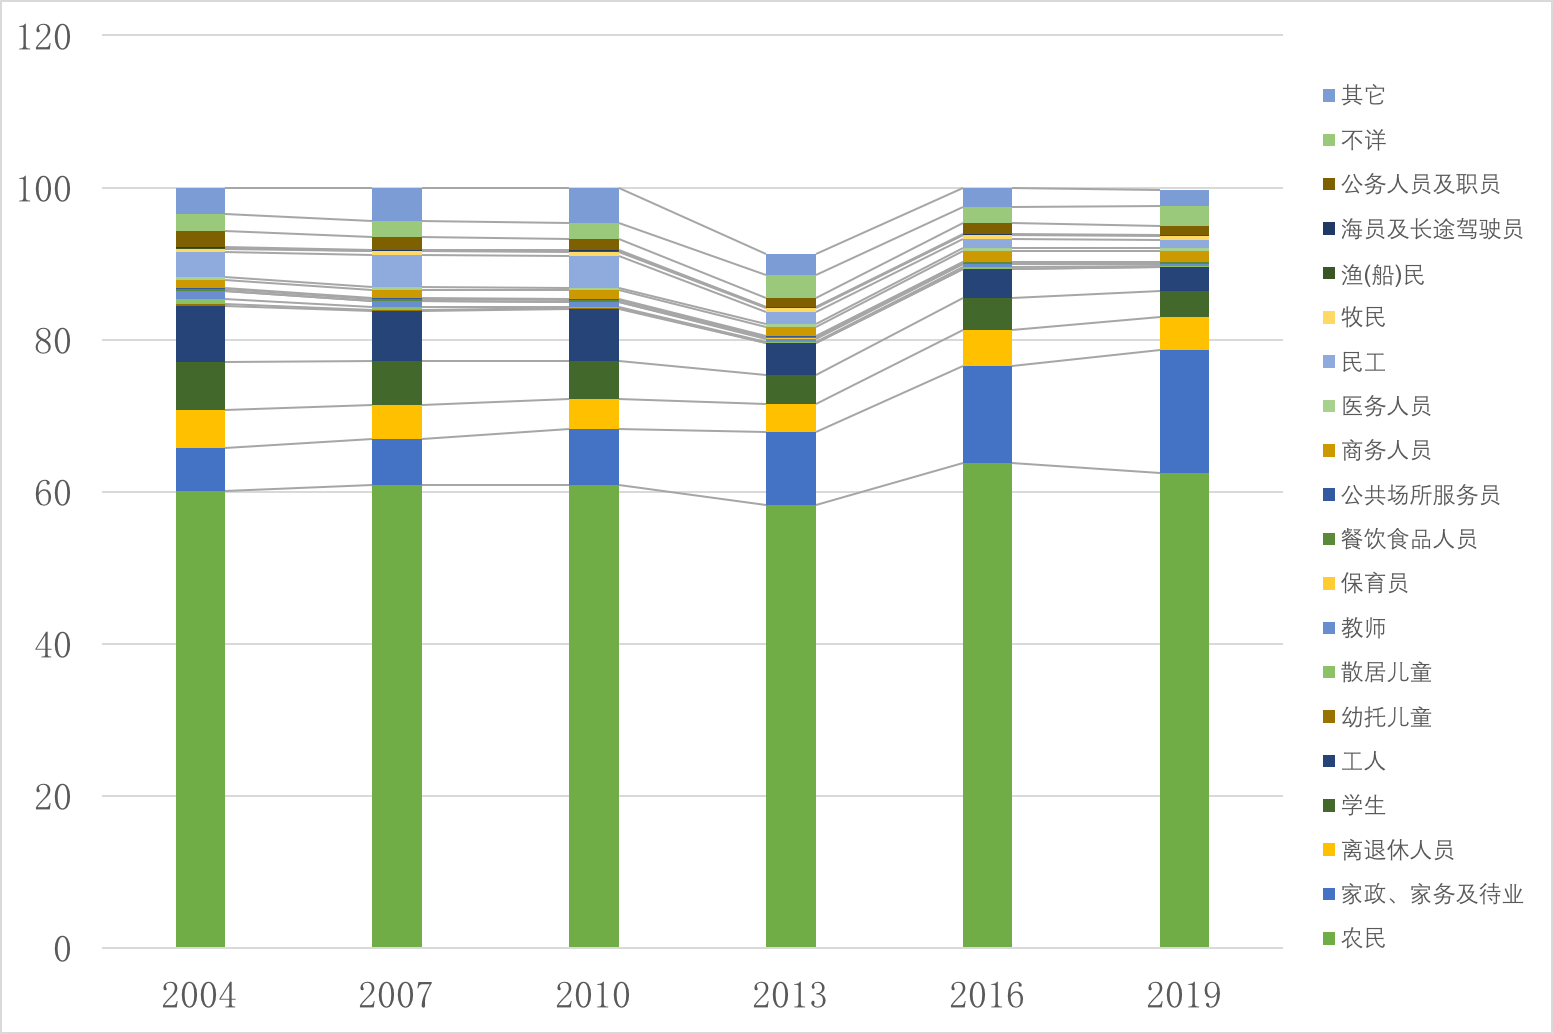
\includegraphics[width=.9\textwidth]{4.png}
    \caption{各类型人群发病人数占比}
\end{figure}

由图中我们可以得到,发病人数占比稳定在前三的人群类型是农民、家务家政及待业和离退休人员。与问题分析中的预测趋势相同,说明了有效人群的选取能在一定程度上增加模型预测的精确度。
政府在宣传传染病的预防工作时,应该要对这三种类型的人群引起高度重视,从传染病的最大传播源头

对于防控排名前3名的重点人群,跟随着各指标对应的权重值变化。根据模型建立的三种权重值的典型情况,我们得到结果如下表所示:
\begin{table}[H]
    \caption{不同权重值对应的防控前3重点人群} \centering 
    \begin{tabular*}{13cm}{ccccccc}
        \toprule[1.5pt]
        权重值 & 重点人群 \\
        \midrule[1pt]
        $w_{1i}=0.3,w_{2i}=0.7$ &  \\
        $w_{1i}=w_{2i}=0.5$ &  \\
        $w_{1i}=0.7,w_{2i}=0.3$ & \\
        \bottomrule[1.5pt]
    \end{tabular*}
\end{table}
根据不同的防控标准,我们得到不同的重点人群。同时发现,当权重值发生变化时,存在 此种类依然是防控前3,说明该类行人群受到权重影响不大,容易受到传染病影响。

\subsubsection{重点区域预测结果} 
由表格可知,均方误差根控制在 以下,平均相对误差控制在 以下,预测模型精确度较高,数据拟合程度较好。
对发病人数占比和死亡率进行模型精度的检验,分别求解MSE和MAPE结果如下表所示:
\begin{table}[H]
    \caption{模型精度检验指标} \centering 
    \begin{tabular*}{8cm}{ccccc}
        \toprule[1.5pt]
         & MSE & MAPE \\
         \midrule[1pt]
         发病人数占比 &  &  \\
         死亡率 & & \\
         \bottomrule[1.5pt]
    \end{tabular*}
\end{table}
灵敏度是判断一个规划函数中参数变化对模型的影响,最常见的灵敏度分析是对目标系数的变化和约束条件的影响。在本题中,约束条件是迭代次数或误差值精度,因此对目标系数的灵敏度分析如下:

\section{问题三模型的建立与求解}
\subsection{问题分析}
问题三在问题二的基础上,需要考虑经济发展对传染病发病人数和死亡人数的影响。我们选取了居民消费支出和人均医疗卫生机构数量\textsuperscript{\cite{bib:eleven}}来对传染病预测模型进行改进。

居民消费支出是指城乡居民个人和家庭用于生活消费以及集体用于个人消费的全部支出,反映的是总体水平的提高对个体的影响,通过消费的物质产品和劳务的数量和质量反映出来。省份经济发展必然会对医疗设施的提高产生影响,因此我们选取此项指标对治疗传染病防控方面作出评价。

人均医疗卫生机构数量是指每个省份居民个人所拥有的能够从事疾病诊断、治疗活动的卫生机构数量,正面反映了一个省份的传染病控制能力,体现了个体指标对传染病的控制水平。

\subsection{问题三模型的建立}
根据问题二的小生境传染病传播模型基础,我们将从地区经济发展中医疗条件的角度对本传染病传播模型进行修正。
问题分析中的两个指标加入小生境的个体属性中记为$c,d$,更改个体变化规则如下:
\begin{equation*}
    f_q=k_1cos(\omega_a\alpha_b)+k_2sin(\omega_a\alpha_b)+2k_3cos(2\omega_a\alpha_a)+2k_4cos(2\omega_b\alpha_b), 
\end{equation*}
\begin{equation*}
    f_p=k_5(\omega_a)^3+k_6(\alpha_a)^2+k_7(\beta_a)+k_8,
\end{equation*}
\begin{align}
    f_m=k_{9}cos(w_cx_c)+k_{10}sin(w_cx_c)+k_{11}cos(2w_cx_c)+k_{12}sin(2w_cx_c)\\
    \notag
    +k_{13}cos(3w_cx_c)+k_{14}sin{3w_cx_c}+k_7x_c^3+k_{15}x_c^2+k_{16}x_c+k_{17},
\end{align}
\begin{align}
    f_n=k_{18}cos(w_dx_d)+k_{19}sin(w_dx_d)+k_{20}cos(2w_dx_d)+k_{21}sin(2w_dx_d)\\
    \notag
    +k_{22}cos(3w_dx_d)+k_{23}sin{3w_dx_d}+k_{24}x_d^3+k_{25}x_d^2+k_{26}x_d+k_{10},
\end{align}
\begin{equation}
    f=\frac{f_q+f_p+f_m+f_n}{k_{27}L_{\omega\alpha}},
\end{equation}
其中在原个体属性的基础上,新增了规则$f_m,f_n$,表示个体属性中人均医疗卫生机构指标和居民消费支出指标,$w_c,x_c;w_d,x_d$分别表示针对两个指标使用傅里叶级数拟合得到的两组趋势描述子,
$k_i,i=1,2,\dots,27$,表示变化规则中的拟合系数。

\subsection{模型求解与结果检验}
\subsubsection{预测结果}

\subsubsection{结果检验}  
在改进预测模型之后对对发病人数和死亡率进行模型精度的检验,分别求解MSE和MAPE结果如下表所示:
\begin{table}[H]
    \caption{模型精度检验指标} \centering 
    \begin{tabular*}{8cm}{ccccc}
        \toprule[1.5pt]
         & MSE & MAPE \\
         \midrule[1pt]
         发病人数占比 &  &  \\
         死亡率 & & \\
         \bottomrule[1.5pt]
    \end{tabular*}
\end{table}
与问题二相比,可以得到模型的精确度提升了,说明添加经济发展因素对传染病预测模型有促进作用。在对模型进行改进与推广时,可以首先结合预测地区经济发展水平的分析\textsuperscript{\cite{bib:twelve}},对模型进行实际意义的改进,再通过对预测原理的分析,减少模型误差。
\section{给相关部门的一封建议信}
\noindent 尊敬的政府工作人员:

你们好!随着科学技术的不断发展,人民生活水平不断提高,同时也伴随着因为生活习惯和的确发展不平衡导致的传染病不断传播。因此,我认为政府部门提前做好传染病预测工作,对于城市经济发展是十分有必要的。

传染病是指由病原微生物(病毒、细菌、真菌、螺旋体、衣原体、支原体、立克次体和寄生虫)感染人或其他生物后产生的,具有传染性并在一定条件下可造成流行的疾病。有史以来,传染病就对人类的生存和健康构成了极大的威胁。面对近些年来来势汹汹的各种传染病,我们不仅要了解它们的发病原因、传播途径和方式,还需要知道它们的传播过程的内在规律,从而才能更好地预防、控制它们。
随着社会进步和医疗技术的发展,人类在和传染病的斗争中也取得了辉煌的成果。

考虑到流行病在温带地区都表现出强烈的季节性波动,具体表现在疾病的发病率和死亡率上。因此,政府部门在控制预防传染病时,采用通过预测发病人数和死亡人数来控制疫情的传播,同时也能有效减少因缺少对传染病传播程度的认知而导致的公众恐慌。

结合历史数据和模型预测的2019年传染病的发病人数和死亡人数,我们发现二者都呈现下降趋势,说明我国政府在传染病病情控制上取得了很好的效果。

从地区分布上来看,传染病主要分布在人群密度较大的省份例如广东省、广西省和重庆,这些地方由于具有地理、人文旅游等优势,每年会吸引大量的外地游客,使得其人口密度在一段时间内会呈现迅速增长,在此时期内有利于传染病的传播。
传染病同时也在偏远地区例如新疆、贵州等省份的发病人数、死亡率较高,这些地区虽然地域辽阔、人口密度低,但是由于自然环境恶劣,基础医疗设施相比于其它省份确实很多,因此,传染病出现疫情后不能得到有效控制,不利于人群的即时防控。

从人群类型上看,农民和家政家务及待业的发病人数占比相比于其它类型的人群相对较高,这侧面说明了在农民的生活环境或是生活习惯有利于传染病的传播。因此,政府部门应该深入探究农民的

政府在流行病爆发时,可以采取的主要的医疗控制手段有注射疫苗、隔离防治、药物治疗等\textsuperscript{\cite{bib:thirteen}}。疾病爆发后,群众也应该自发地采取少去人群密集的公共区域、购买增强对疾病抵抗力的药物等措施。
但对于一些新的传染病或是以及存在的但又发生新的变异的传染病,传统的治疗方案可能作用有限,需要医疗专家找到新的方案,这期间耗费的时间政府也需要考虑。
当今,注射疫苗是控制传染病最直接最有效的方法,但一般而言,一种新的传染病出现需要 3 个月的时间研发、量产新的疫苗。
这些在我们研究疾病内在机理、采取控制措施、构建数学模型时都应该考虑进去(有些因素影响力较小,在构建模型时可以省去)。
在传染病防控的措施上,建立合适的模型,结合相关理论知识,传染病专家可以发现疾病的传播规律和发展趋势并依此找到更好的预防和控制方案,从而最大程度地减少人民群众的生命财产损失,这是每个政府部门应该承担起的责任。

\section{模型评价}

\subsection{模型优点}
(1)利用三次多项式回归模型对非线性动态时间序列的强拟合能力,构建基于三次多项式回归模型的预测传染病预测模型P-GM(1,1),提高了对于传染病发病人数和死亡人数预测的准确性。

(2)
\subsection{模型缺点}
(1)

(2)
\subsection{模型改进}
(1)在问题一的P-GM(1,1)模型中,预测值与实际值仍然存在偏差,这些偏差形成的残差数列能够通过波动性较强的马尔科夫链(Markov chain)对P-GM(1,1)模型进行再次改进以进一步提升本文所建模型对于动态云计算负荷时间序列的拟合能力,构建MP-GM(1,1)模型。

(2)
\begin{thebibliography}{9}
    \bibitem{bib:one} Rashid Tarik A,Abbas Dosti K,Turel Yalin K. A multi hidden recurrent neural network with a modified grey wolf optimizer.[J]. PloS one,2019,14(3).
    \bibitem{bib:two} 郭琳. 2012-2016年某市宽城区法定传染病监测分析及防控策略研究[D].吉林大学,2018.
    \bibitem{bib:three} Walker Rachel A,Wright Kristina J,Jhou Thomas B,McDannald Michael H. The ventrolateral periaqueductal gray updates fear via positive prediction error.[J]. The European journal of neuroscience,2019.
    \bibitem{bib:four} Pumei G,Jun Z,Jiefang L,Ines Tejado Balsera. Fractional-Order Accumulative Linear Time-Varying Parameters Discrete Grey Forecasting Model[J]. Mathematical Problems in Engineering,2019,2019.
    \bibitem{bib:five} Jacob J. Hadle,F. Leland Russell,James B. Beck. Are buffalograss ( Buchloë dactyloides ) cytotypes spatially and ecologically differentiated?[J]. American Journal of Botany,2019,106(8).
    \bibitem{bib:six} 晁童. 基于小生境遗传算法的定量关联规则算法研究[D].西安理工大学,2018.
    \bibitem{bib:seven} Alwin A. Hardenbol,Timo Pakkala,Jari Kouki. Persistence of a keystone microhabitat in boreal forests: Cavities of Eurasian Three-toed Woodpeckers ( Picoides tridactylus )[J]. Forest Ecology and Management,2019,450.
    \bibitem{bib:eight} 何华. 基于时间影响网络的传染病应急方案评价与调整方法[D].国防科学技术大学,2014.
    \bibitem{bib:nine} 覃柳麻. 2012-2017年南宁市乙肝流行特征及空间分析[D].广西医科大学,2019.
    \bibitem{bib:ten} R. Bretin,M. Levesque,P. Bocher. Neighborhood effect on the strain distribution in linearly elastic polycrystals: Part 2 – Cellular Automaton[J]. International Journal of Solids and Structures,2019,176-177.
    \bibitem{bib:eleven} Azath Mubarakali,Jayabrabu Ramakrishnan,Dinesh Mavaluru,Amria Elsir,Omer Elsier,Karzan Wakil. A new efficient design for random access memory based on quantum dot cellular automata nanotechnology[J]. Nano Communication Networks,2019,21.
    \bibitem{bib:twelve} Babaie Javad,Ardalan Ali,Vatandoost Hasan,Goya Mohammad Mahdi,Akbarisari Ali. Communicable Disease Surveillance Systems in Disasters: Application of the Input, Process, Product, and Outcome Framework for Performance Assessment.[J]. Disaster medicine and public health preparedness,2019,13(2).
    \bibitem{bib:thirteen}尉景辉. 面向传染病监测的互联网情报动态跟踪系统研究[D].中国人民解放军军事医学科学院,2015.
\end{thebibliography}

\section{代码}
\subsection{全国发病人数和死亡人数的时间关联性检验--Matlab 源程序}
\begin{lstlisting}[language=Matlab]
    maindata =kafang;
    [m,k]=size(maindata);
    tt=[];Varr=[];Uu=[];Pcount=[];
    %% 计算卡方检验,并求出各项指标
    for icount=1:k-1
        y=[maindata(:,1),maindata(:,icount+1)];
        n = length (y);
        s = 0;
        for j =1:n
          for i =1:j
                if y(i)<y(j)
                  s = s +1;
                else
                  s = s;
                end
          end
            p = s;
        end
        pcount=[Pcount,p];
        t=4*p/(n*(n-1))-1;
        tt=[tt,t];
        Var=2*(2*n+5)/(9*n*(n-1));
        Varr=[Varr,Var];
        U=t/sqrt(Var);
        Uu=[Uu,U];   
    end
    t,Var,U
\end{lstlisting}


\end{document}